\documentclass[a4paper,12pt]{article}
\usepackage{amsmath}
\usepackage{graphicx}
\usepackage[margin=1in]{geometry}
\begin{document}

\title {Changing frame of reference}
\maketitle
		

\section{Change reference frame}

Suppose you have a mass M on an inclined slope, 30 degrees up from the horizon. The mass is supported in place by a string with Tensile Force T.
\begin{figure}[htbp]
\centering
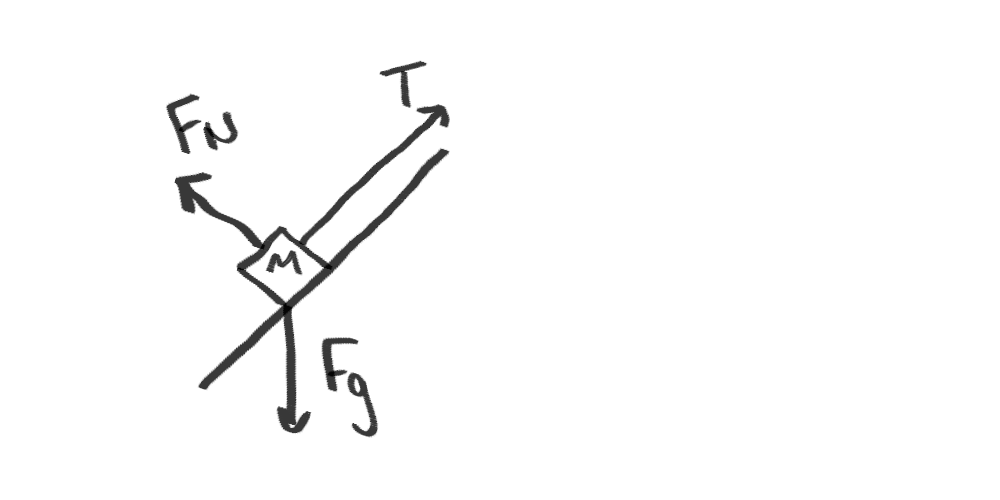
\includegraphics[width=1.0\textwidth]{FBD.png}
\end{figure}




\begin{enumerate}
	\item{Write out the two x and y equations of motion in the usual x-y coordinate system, knowing that the block is stationary.}
	\item{If only the mass were specified, say $M = 50kg$, would you be able to use just one equation to solve for either the tensile force or the normal force?}
		\newpage
	\item{Consider this new coordinate system, with $\alpha$ replacing $x$ and $\beta$ replacing $y$.
		\begin{figure}[htbp]
\centering
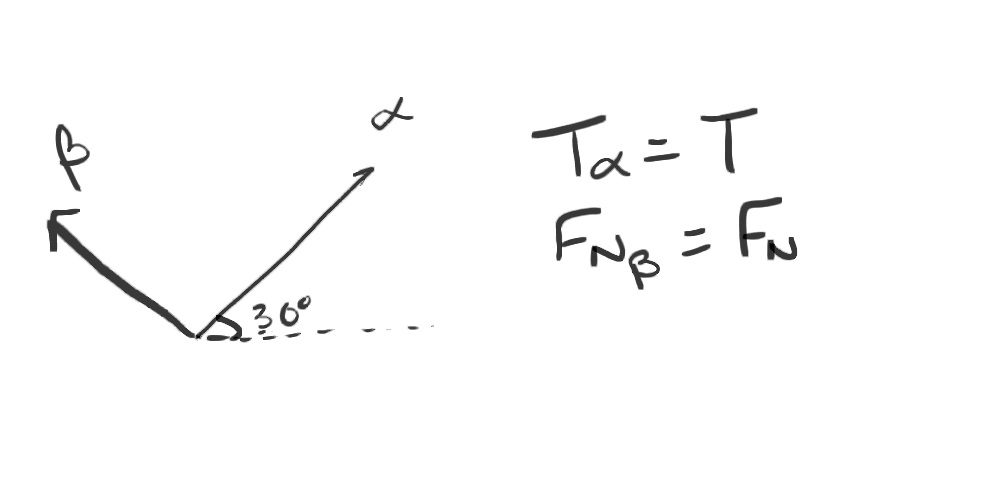
\includegraphics[width=1.0\textwidth]{newcoords.jpg}
\end{figure}
		\newline
		Note that in this coordinate system, $T_{\alpha} = T$ because T is perfectly in line with the alpha axis. $F_{N\beta} = F_N$ because the normal force is perfectly in line with the beta axis. Rewrite the two equations of motion for the alpha and beta axes. For instance, $\Sigma F_{alpha} = 0 = T - F_{g \alpha}.$ What is the $\beta$ equation?}	\item{If only the mass were specified as $M = 50kg$ and you didn't know the tensile force or the normal force, solve for them. }

\end{enumerate}
\section{BONUS}
In either coordinate system we have two equations and two unknowns, which means we have enough information to completely solve it, but it wasn't as easy in the x-y coordinate system. Can you find an expression for $F_N$ in the x-y coordinate system?
\end{document}
